\documentclass[12pt]{article}
\usepackage{graphicx}
\usepackage[margin=30mm, paper = a4paper]{geometry}
\usepackage{minted}
\usepackage{multicol}
% \usepackage[english]{babel}

\title{Basic MySQL Operations}
\author{Md Tajim An Noor}
\date{}

\begin{document}
\vspace*{\fill}
\begin{center}

    \emph{Heaven's Light is Our Guide} \\
    \textbf{Rajshahi University of Engineering and Technology} \\

    \begin{figure}[h]
        \centering
        
\includegraphics[scale=.34]{images/RUET_logo.png}
        \label{fig:ruet_logo}
    \end{figure}
    \vspace{5mm}

    \textbf{Course Code}\\
    ECE 2216\\
    \vspace{3mm}
    \textbf{Course Title}\\
    Database Systems Sessional

    \vspace{5mm}
    \textbf{Experiment Date:} October 15, 2023,\\
    \textbf{Submission Date:} November 5, 2023\\

    \vspace{5mm}
    \textbf{Lab Report 3:} Creating a database and doing operations on it using SQL\\

    \vspace{15mm}

    \begin{tabular}{c|c}
        \textbf{Submitted to} & \textbf{Submitted by} \\
        Md. Robiul Islam      & Md. Tajim An Noor     \\
        Assistant Professor   & Roll: 2010025         \\
        Dept of ECE, Ruet     &                       \\
    \end{tabular}

\end{center}
\vspace*{\fill}

\pagebreak

\tableofcontents

\maketitle

\section{Tools Used}
\begin{itemize}
    \item MySQL
    \item VS Code - as an IDE to use SQL
    \item MacTeX -\LaTeX  compiler
    \item VS Code with LaTeX workshop extension as a text editor
\end{itemize}


\section{Process}
\subsection{SQL Codes:}

\vspace{10mm}

\subsubsection{Create a orderdetails table orderdetails(order\_no, customer\_no, address, product\_category, quantity, unit\_price):}
\subsubsection*{Code: }
\begin{minted}[breaklines, linenos]{mysql}
    CREATE DATABASE if NOT EXISTS ProductOrder;
    use ProductOrder;
    create TABLE
        OrderDetails (
            Order_No int AUTO_INCREMENT primary key,
            CustomerName varchar(30),
            Address_ varchar(300),
            ProductCatagory varchar(20),
            Quantity int,
            UnitPrice decimal(8, 2)
        )     
\end{minted}
Here a new database named ProductOrder. Then with the $Use$ command, the database was selected and then using Create Table, a new table was created as asked.

\subsubsection{Add a cloumn named order\_date that expresses the ordered date:}
\subsubsection*{Code: }
\begin{minted}[breaklines, linenos]{mysql}
    ALTER TABLE ProductOrder.OrderDetails ADD OrderDate DATETIME after UnitPrice
\end{minted}
Here, using the ALTER TABLE clause, a new column, which wasn't added in during the CREATE TABLE clause, is added at the end of the table.

\vspace{13mm}

\subsubsection{Rename the column customer\_name to cust\_name.}
\subsubsection*{Code:}
\begin{minted}[breaklines, linenos]{mysql}
    ALTER TABLE ProductOrder.OrderDetails change CustomerName Cust_name varchar(30);
\end{minted}
Same as 2.1.2, ALTER TABLE clause was used to modify a column's name.

\vspace{13mm}

\subsubsection{Drop the product\_category column and recreate the column.}
\subsubsection*{Code:}
\begin{minted}[breaklines, linenos]{mysql}
    ALTER TABLE ProductOrder.OrderDetails
    drop column ProductCatagory;

    ALTER TABLE ProductOrder.OrderDetails ADD ProductCatagory varchar(20) after Address_;
\end{minted}
Here too, ALTER TABLE clause was used to modify the table. We first dropped the column and then inserted it into the same place.

\vspace{13mm}

\subsubsection{Keep the orde\_no as auto increment column.}
To do this, the line no. 7 in 2.1.1 was used. While creating the table, the column was declared as PRIMARY\_KEY and another attribute: AUTO\_INCREMENT was added right there.

\vspace{13mm}

\subsubsection{Now insert at least 15 rows into the table.}
\subsubsection*{Code:}
\begin{minted}[breaklines, linenos]{mysql}
    INSERT INTO
    ProductOrder.OrderDetails (
        Cust_name,
        Address_,
        ProductCatagory,
        Quantity,
        UnitPrice,
        OrderDate
    )
    VALUES
    (
        'Rahul',
        'Talaimari',
        'Home Appliances',
        4,
        '3000.00',
        now ()
    ),
    ...
    ...
\end{minted}
Using the INSERT INTO clause, 15 different entity was entered into the table. (To save space, only two instances of the code is shown here.)

\vspace{13mm}

\subsubsection{Show the orderdetails  in ascending order based on the quantity.}
\subsubsection*{Code:}
\begin{minted}[breaklines, linenos]{mysql}
    SELECT
    *
    FROM
        ProductOrder.OrderDetails
    ORDER BY
        Quantity ASC;
\end{minted}
Using the select clause, this task was done. The $*$ selects all the data in the table and ORDER BY clause defines how to show the table.

\vspace{13mm}

\subsubsection{Show the orderdetails  in descending order based on the uni\_price}
\subsubsection*{Code:}
\begin{minted}[breaklines, linenos]{mysql}
    SELECT
    *
    FROM
        ProductOrder.OrderDetails
    ORDER BY
        UnitPrice DESC;
\end{minted}
Same as the last task, only difference was here the ORDER BY was done in descending order.

\vspace{13mm}

\subsubsection{Show the order\_no, cust\_name, address and unit\_price  in ascending order based on the 10\% increment in unit\_price.}
\subsubsection*{Code:}
\begin{minted}[breaklines, linenos]{mysql}
    SELECT
        Order_No,
        Cust_name,
        Address_,
        UnitPrice+UnitPrice*.1 as New_Price
    FROM
        ProductOrder.OrderDetails
    ORDER BY
        UnitPrice DESC;
\end{minted}
By formatting in the SELECT clause, the UnitPrice column was shown differently as wanted. Then usinf the ORDER BY clause, the sorting was done.

\vspace{13mm}

\subsection{Output}
\begin{figure}[H]
    \centering
    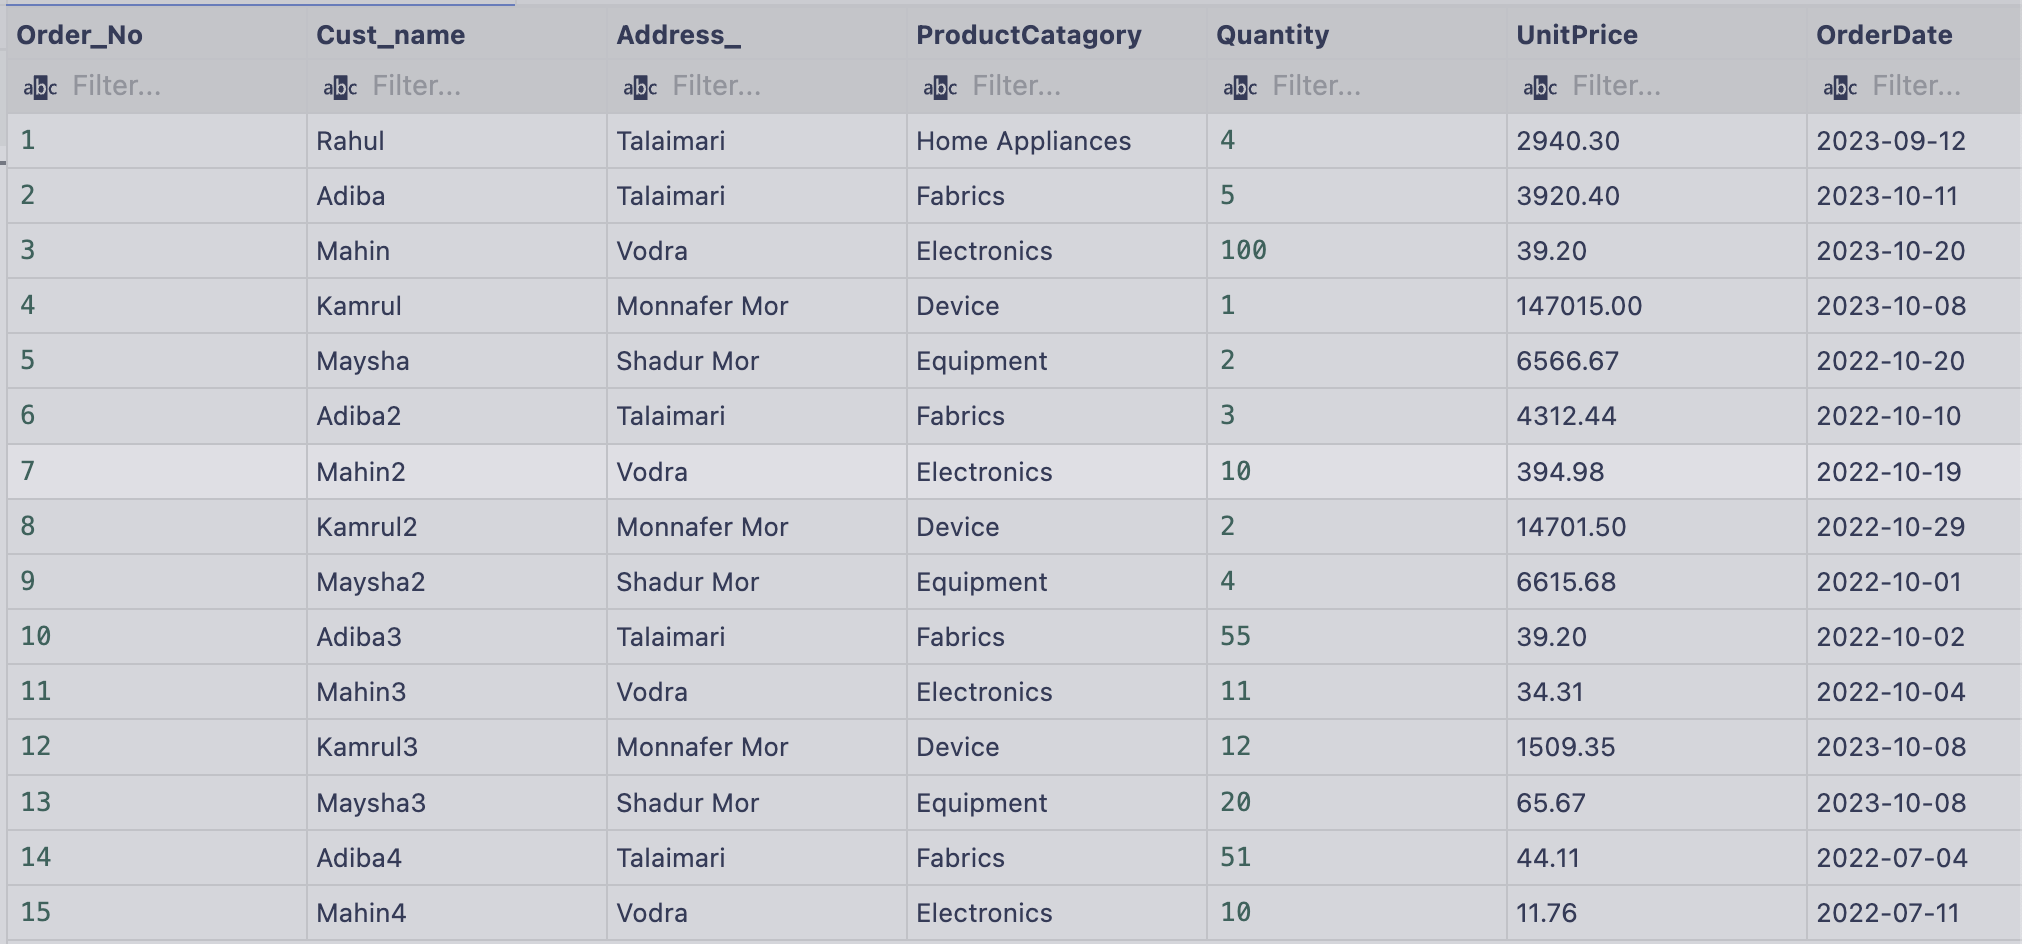
\includegraphics[width=\textwidth]{images/1full.png}
    \caption{Table of Product Order Details}
    \label{fig:table}
\end{figure}
\begin{figure}[H]
    \centering
    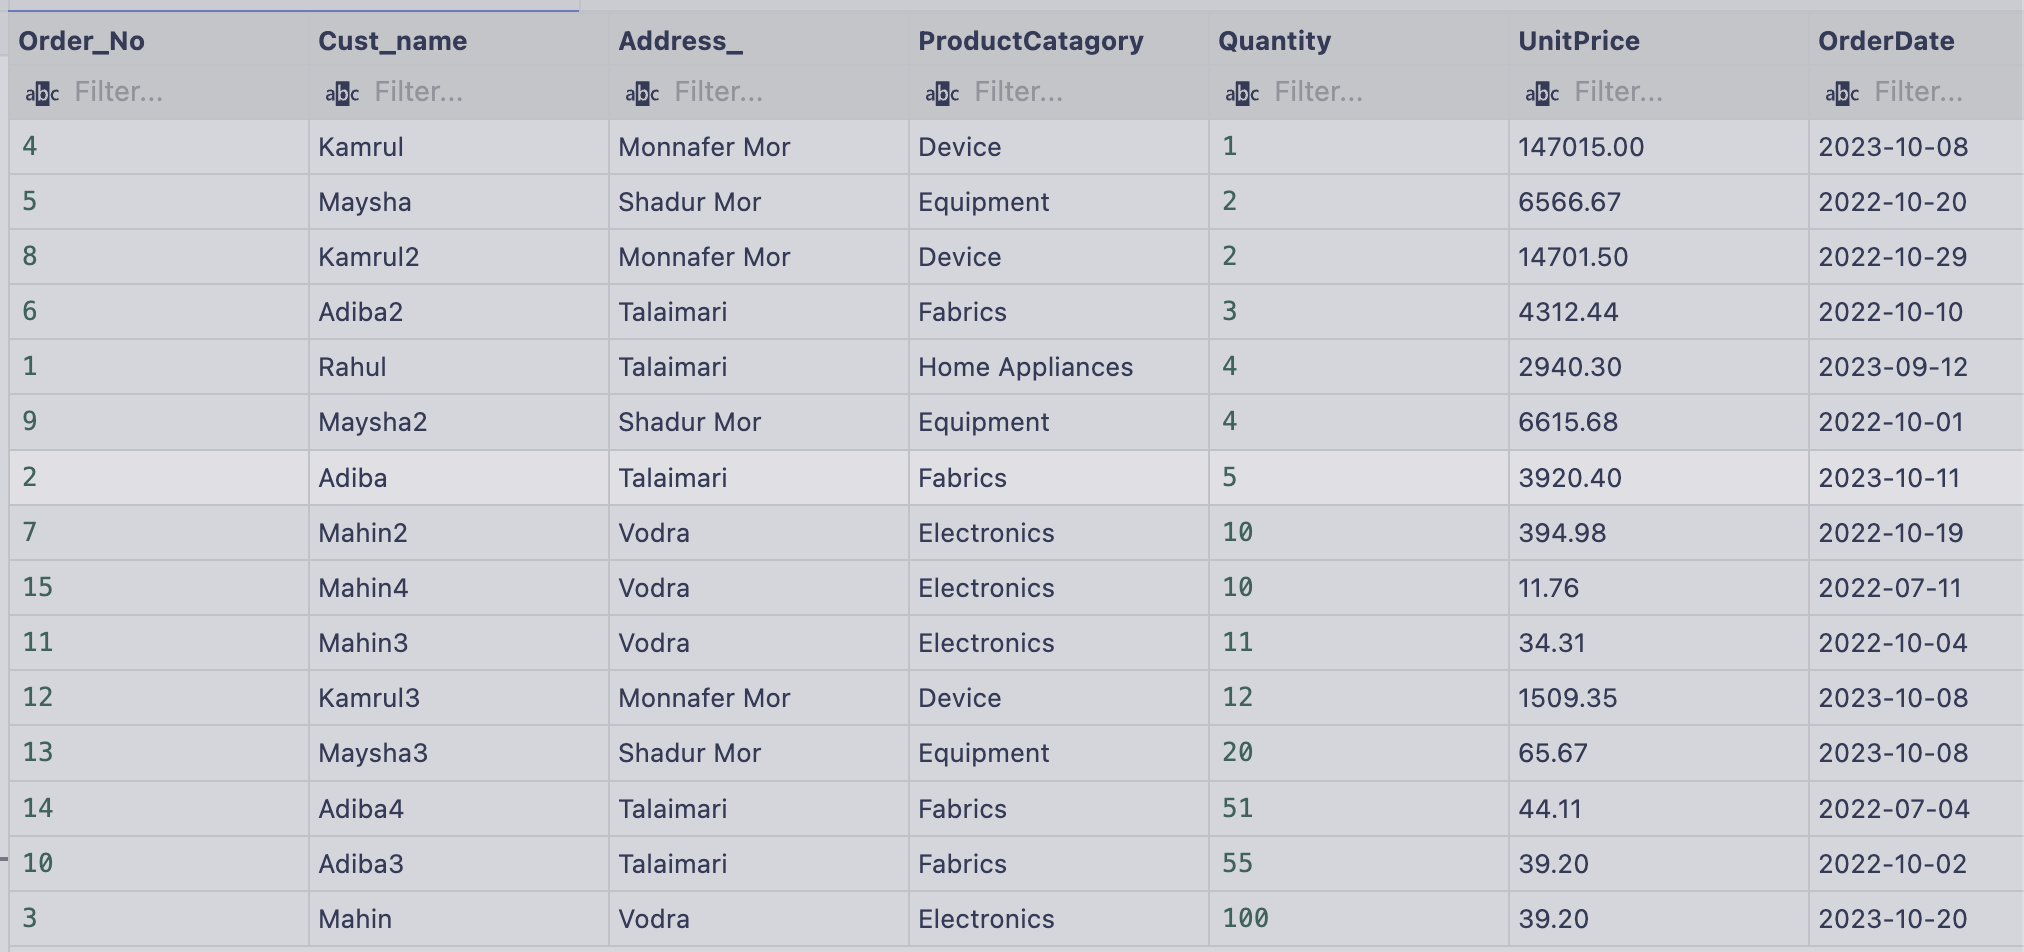
\includegraphics[width=\textwidth]{images/2sortQuan.png}
    \caption{Table sorted in ascending order of Quantity}
    \label{fig:sort1}
\end{figure}
\begin{figure}[H]
    \centering
    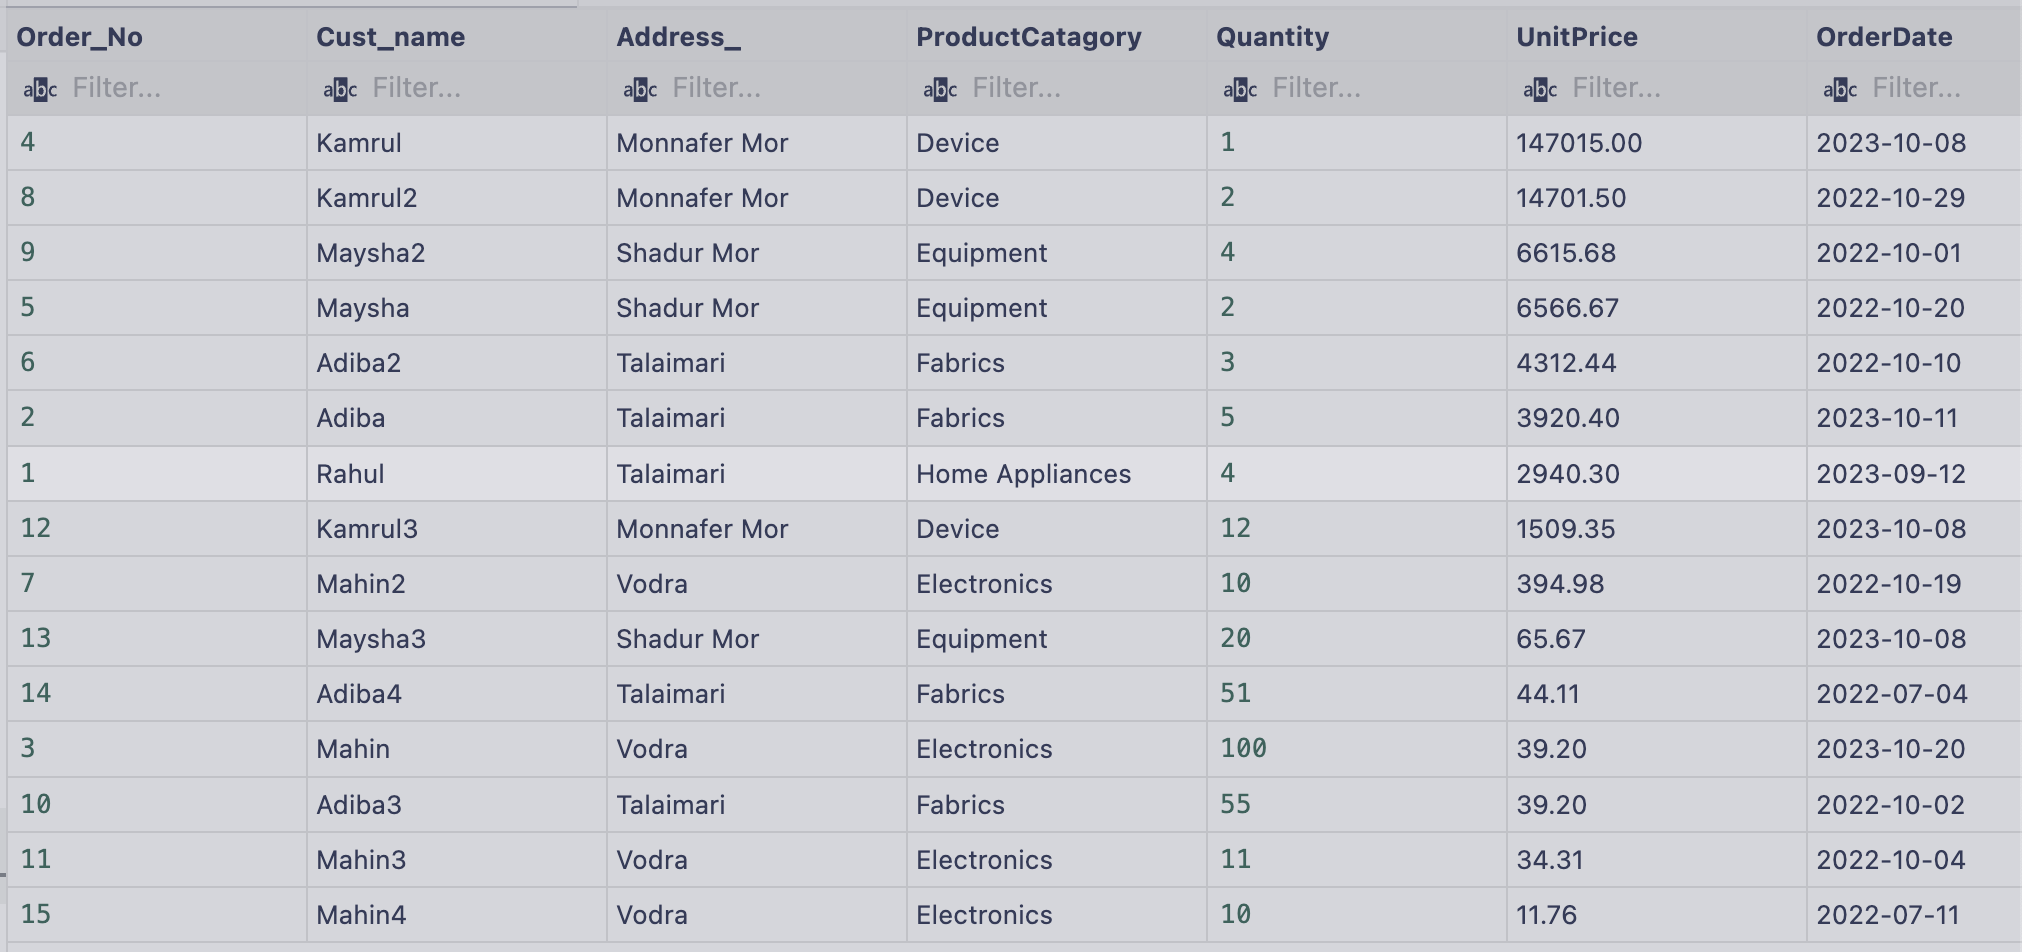
\includegraphics[width=\textwidth]{images/3sortUnit.png}
    \caption{Table sorted in descending order of UnitPrice}
    \label{fig:sort2}
\end{figure}
\begin{figure}[!ht]
    \centering
    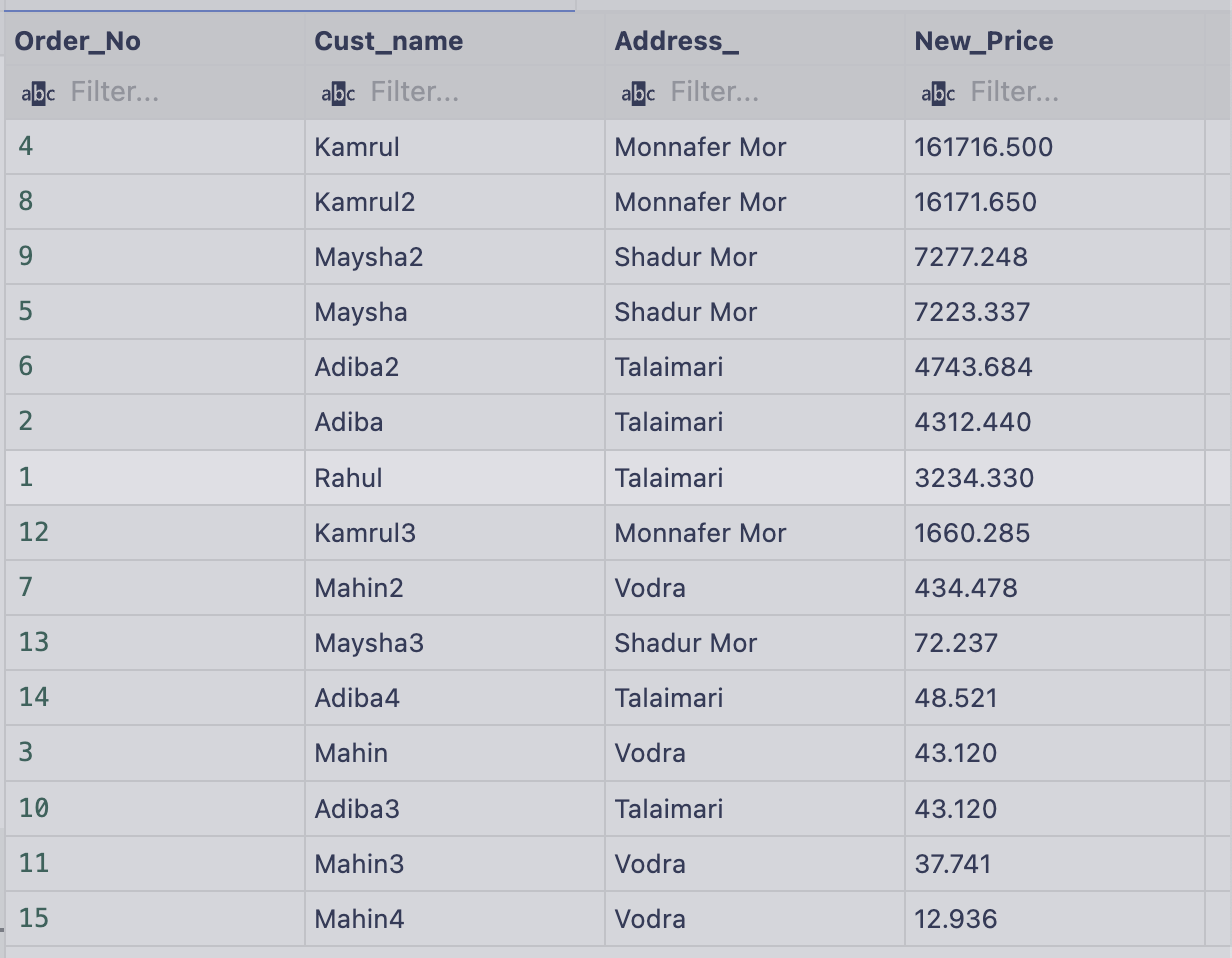
\includegraphics[width=\textwidth]{images/4query.png}
    \caption{Table query with edit in UnitPrice}
    \label{fig:query}
\end{figure}

% \bibliographystyle{IEEEtran}
% \bibliography{ref}
\end{document}